\documentclass[a4paper]{article}
\setlength{\parindent}{0pt}

%%%%%%%% CREATE DOCUMENT STRUCTURE %%%%%%%%
%% Language and font encodings
\usepackage[english]{babel}
\usepackage[utf8x]{inputenc}
\usepackage[T1]{fontenc}
%\usepackage{subfig}

%% Sets page size and margins
\usepackage[a4paper,top=3cm,bottom=2cm,left=2cm,right=2cm,marginparwidth=1.75cm]{geometry}

\usepackage{tikz}
\usetikzlibrary{arrows, shapes.geometric, intersections}

\tikzstyle{smallbuilding} = [rectangle, rounded corners, minimum width=4cm, minimum height=1.5cm,text centered, draw=black, fill=red!30]
%\tikzstyle{code} = [trapezium, trapezium left angle=70, trapezium right angle=110 , minimum width=3cm, minimum height=1cm, text centered, draw=black, fill=blue!30]
\tikzstyle{mediumbuilding} = [rectangle, minimum width=3cm, minimum height=1cm, text centered, draw=black, fill=green!30]
\tikzstyle{largebuilding} = [rectangle, minimum width=3cm, minimum height=1cm, text centered, draw=black, fill=orange!30]


%% Useful packages
\usepackage{framed}
\usepackage{amsmath}
\usepackage{graphicx}
%\usepackage[colorinlistoftodos]{todonotes}
\usepackage[colorlinks=true, allcolors=blue]{hyperref}
\usepackage{caption}
\usepackage{subcaption}
\usepackage{listings}
\usepackage{lstautogobble}
\usepackage{sectsty}
\usepackage{apacite}
\usepackage{float}
\usepackage{titling} 
\usepackage{blindtext}
\usepackage[square,sort,comma,numbers]{natbib}
\usepackage{xcolor}
\definecolor{darkgreen}{rgb}{0.0, 0.4, 0.0}

\definecolor{pblue}{rgb}{0.13,0.13,1}
\definecolor{pgreen}{rgb}{0,0.5,0}
\definecolor{pred}{rgb}{0.9,0,0}
\definecolor{pgrey}{rgb}{0.46,0.45,0.48}

\usepackage{listings}
%\lstset{language=Java,
%    showspaces=false,
%    showtabs=false,
%    breaklines=true,
%    showstringspaces=false,
%    breakatwhitespace=true,
%    commentstyle=\color{pgreen},
%    keywordstyle=\color{pblue},
%    stringstyle=\color{pred},
%    basicstyle=\ttfamily,
%    colframe=white!75!black,
%    moredelim=[is][\textcolor{pgrey}]{\%\%}{\%\%}
%}

\usepackage[most]{tcolorbox}

\newtcblisting{shell}{colback=black,colupper=white,colframe=white!75!black,
	listing only,listing options={language=sh}}

% ToDo: List
\usepackage{enumitem,amssymb}
\newlist{todolist}{itemize}{2}
\setlist[todolist]{label=$\square$}

%%%%%%%% DOCUMENT %%%%%%%%
\begin{document}

%%%% Title Page
\begin{titlepage}

\newcommand{\HRule}{\rule{\linewidth}{0.5mm}} 							% horizontal line and its thickness
\center 
 
% University
\textsc{\LARGE University of Illinois @ Urbana-Champaign}\\[1cm]

% Document info
\textsc{\Large CI 489: Data Structures for Education}\\[0.2cm]
\textsc{\large }\\[1cm] 										% Course Code
\HRule \\[0.8cm]
{ \huge \bfseries Project 3: Campus Navigator}\\[0.7cm]								% Assignment
\HRule \\[0.8cm]
\vfill
%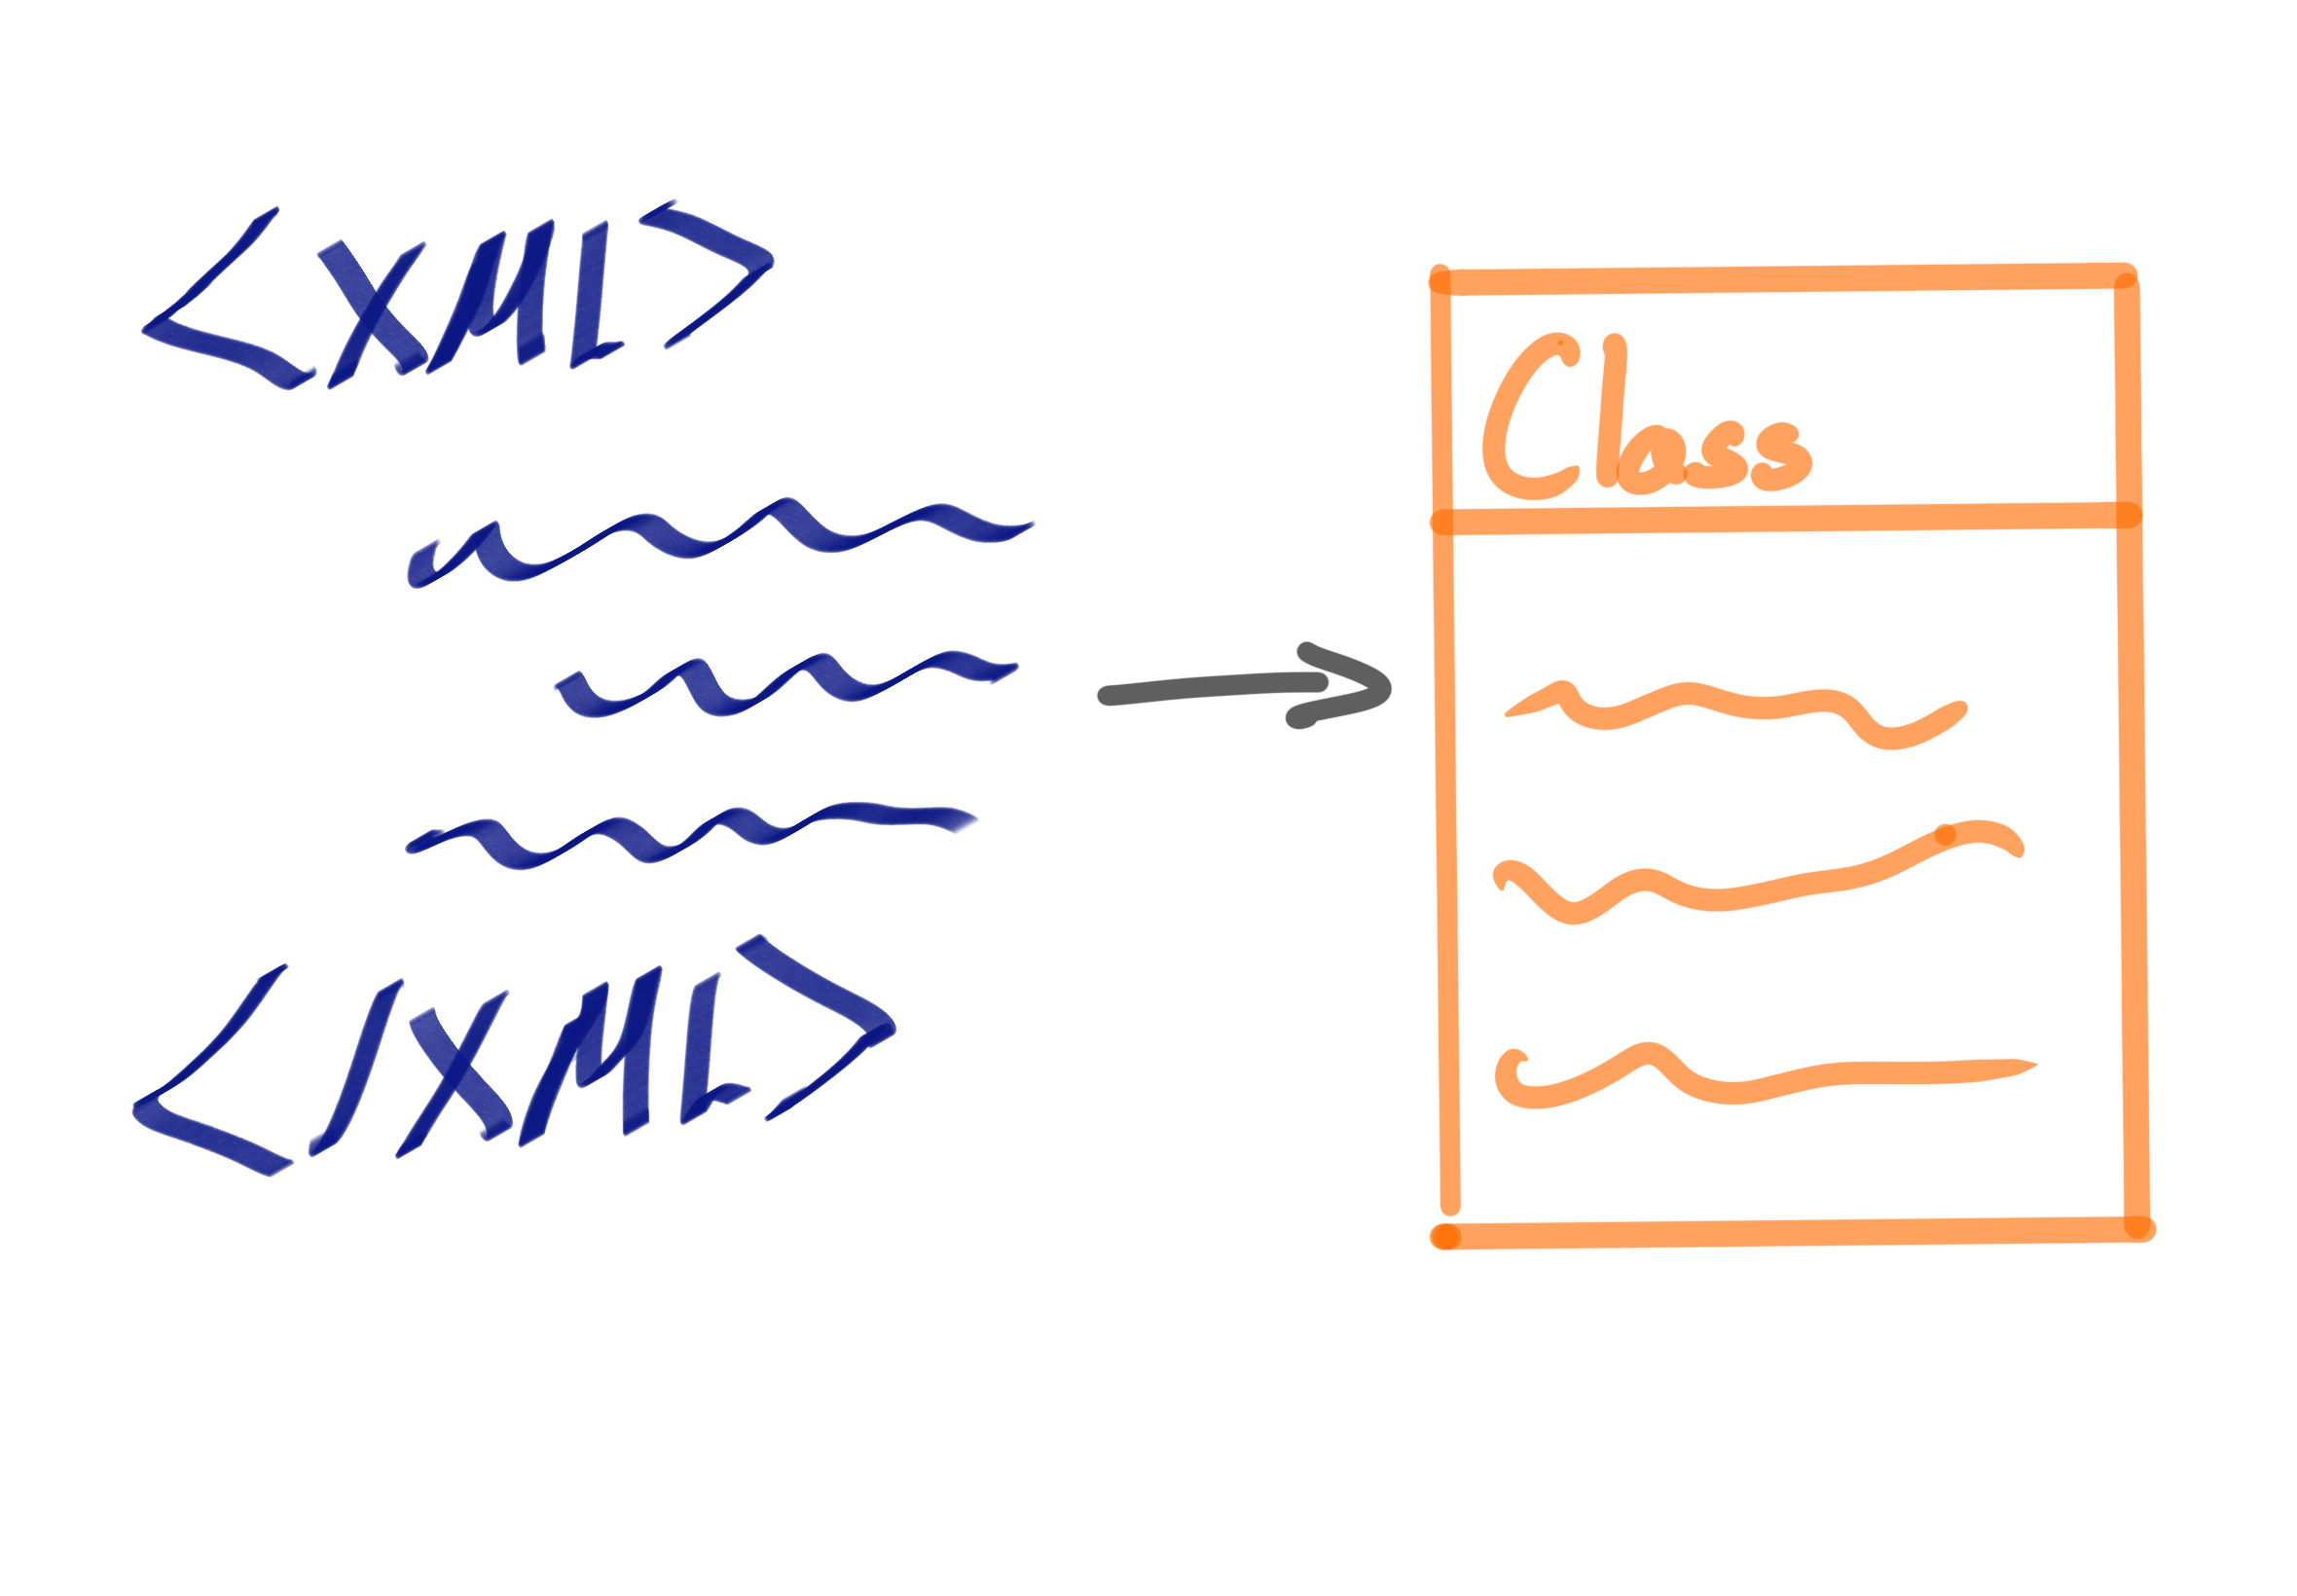
\includegraphics[width=0.6\textwidth]{images/xml.jpg}\\[1cm] 	% University logo
\vfill 
\end{titlepage}


\section*{Objectives and Overview}

\begin{figure}[H]
    \centering

    \resizebox{175px}{!}{%
    \begin{tikzpicture}[node distance=2cm, scale=0.75]

    %Beckman Quad
    \node[main] (beckman) [] {Beckman};

    \node[main] (ece) [below left of=beckman] {ECE};
    \node[main] (nanotech) [below of=ece] {Nanotech. Lab};
    \node[main] (kenny) [below of=nanotech] {Kenny Gym};

    \node[main] (csl) [below right of=beckman] {Coord. Sci. Lab};
    \node[main] (newmark) [below of=csl] {Newmark Lab};
    \node[main] (dcl) [below of=newmark] {Digital Comp. Lab};

    % Bardeen Quad
    \node[main] (englibrary) [below of=dcl] {Grainger Eng. Library};
    \node[main] (cif) [left of=englibrary, node distance=5cm] {Campus Instrct. Facility};
    \node[main] (talbot) [below of=cif, node distance=1.5cm] {Talbot Lab};
    \node[main] (everitt) [below of=talbot] {Everitt Lab};
    \node[main] (mech) [below right of=englibrary] {Mech. Eng. Lab};
    \node[main] (materials) [below of=mech] {Materials Sci.};
    \node[main] (collegeeng) [left of=materials, node distance=2.5cm] {Eng. Hall};

    % Main Quad
    \node[main] (union) [below of=collegeeng, node distance=3cm] {Illini Union};
    \node[main] (altgeld) [left of=union, node distance=4cm] {Altgeld Hall};

    \node[main] (henry) [below of=altgeld] {Henry Admin Bldg};
    \node[main] (english) [below of=henry] {English Bldg};
    \node[main] (lincoln) [below of=english] {Lincoln Hall};

    \node[main] (naturalhist) [right of=union, node distance=3cm] {Natural Hist.};
    \node[main] (noyes) [below of=naturalhist] {Noyes Lab};
    \node[main] (davenport) [below of=noyes, node distance=2.5cm] {Davenport Hall};
    \node[main] (foreign) [below of=davenport, node distance=1.5cm] {Foreign Lang Bldg};

    \node[main] (folinger) [left of=foreign, node distance=3cm, yshift=-1.5cm] {Foellinger Hall};

    % South Quad
    \node[main] (ugl) [below of=folinger] {Undergraduate Lib.};

    \node[main] (morrows) [right of=ugl, node distance=3.5cm] {Morrows Plots};
    \node[main] (mumford) [below of=morrows] {Mumford Hall};

    \node[main] (library) [left of=ugl, node distance=3.5cm] {Library};
    \node[main] (edu) [below of=library, node distance=3.5cm, xshift=-1.5cm] {Education Bldg};
    \node[main] (thbh) [right of=edu, node distance=3cm] {\parbox{2cm}{\centering Temple Hoyne\\ Buell Hall}};
    \node[main] (naturalresc) [below of=edu, xshift=1.0cm] {Natural Resources Bldg};
    \node[main] (stock) [right of=naturalresc, xshift=2.5cm] {Stock Pavilion};
    \node[main] (ag) [below of=mumford, node distance=3cm] {\parbox{2cm}{\centering Ag Eng. \\ Sci. Bldg}};

    %
    % Edges 
    %
    \draw[-] (beckman) -- (ece);
    \draw[-] (beckman) -- (csl);
    \draw[-] (ece) -- (nanotech);
    \draw[-] (nanotech) -- (kenny);
    \draw[-] (csl) -- (newmark);
    \draw[-] (newmark) -- (dcl);
    \draw[-] (kenny) -- (cif);
    \draw[-] (englibrary) -- (cif);
    \draw[-] (dcl) -- (englibrary);
    \draw[-] (cif) -- (talbot);
    \draw[-] (talbot) -- (everitt);
    \draw[-] (everitt) -- (collegeeng);
    \draw[-] (englibrary) -- (mech);
    \draw[-] (mech) -- (materials);
    \draw[-] (materials) -- (collegeeng);
    \draw[-] (everitt) -- (altgeld);
    \draw[-] (everitt) -- (union);
    \draw[-] (materials) -- (union);
    \draw[-] (materials) -- (naturalhist);
    \draw[-] (union) -- (altgeld);
    \draw[-] (union) -- (naturalhist);
    \draw[-] (altgeld) -- (henry);
    \draw[-] (henry) -- (english);
    \draw[-] (english) -- (lincoln);
    \draw[-] (naturalhist) -- (noyes);
    \draw[-] (noyes) -- (davenport);
    \draw[-] (davenport) -- (foreign);
    \draw[-] (lincoln) -- (folinger);
    \draw[-] (foreign) -- (folinger);
    \draw[-] (folinger) -- (ugl);
    \draw[-] (ugl) -- (library);
    \draw[-] (ugl) -- (morrows);
    \draw[-] (library) -- (edu);
    \draw[-] (library) -- (thbh);
    \draw[-] (edu) -- (naturalresc);
    \draw[-] (thbh) -- (naturalresc);
    \draw[-] (edu) -- (thbh);
    \draw[-] (naturalresc) -- (stock);
    \draw[-] (morrows) -- (mumford);
    \draw[-] (mumford) -- (ag);
    \draw[-] (ag) -- (stock);

    \end{tikzpicture}}
%    \caption*{The Three Main Quads of Campus}
\end{figure}


\section*{Structures and Specifications}

\section*{Rubric}

\section*{Instructor Notes}

\end{document}
